\section{Simulations}

% \subsection{Implementation notes}
% For the adaptative time steps scheme a choice had to be made when division by 0 were encountered. Some simulations gave a value of $d=0$ i.e.
% \begin{verbatim}
% y1 = RK4_do_onestep(x, t, dt);
% y_tilde = RK4_do_onestep(x, t, dt / 2.0l);
% y2 = RK4_do_onestep(y_tilde, t, dt / 2.0l);
% \end{verbatim}
% gave the same values for y1 and y2. To avoid a division by 0 in the next step of increasing the dt as such
% \begin{verbatim}
% dt = dt * pow(tol / d, 1.0l / (4.0l + 1.0l));
% \end{verbatim}
% a condition (d != 0.0l) was added before this calculation. If (d==0) the dt is kept constant.

\subsection{Transfer orbit}
The first simulations were about simulating the transfer of Webb from a low Earth orbit ar $r_0$ to the L2 Lagrange point at $r_1$ as defined in \autoref{sec:transfer_anal}. 















\subsection{Around Lagrange L2}

We now consider the reduced 3-body problem, like in \ref{sec:3body_reduced}. The simulations are done in the \(\mathcal R'\) reference frame, placing Webb at the Lagrange L2 point given in \ref{sec:lagrange_L2} and giving the satelite an initial downwards speed \(\dot y' = -0.1\) m/s. In this sections, the simulations are done until \(t_\textrm{fin} = 2\) years. The trajectory of the satelite is given in \autoref{fig:lagrange_trajectory} and will be discussed later. We will first analyse the convergence of both methods.

Due to the nature of the adaptative timestep method, the convergence order against \(\frac{1}{n_\textrm{steps}}\) will be analysed. The results wit the initial conditions given above are reported in \autoref{fig:lagrange_conv}. Both methods converge with order 5 to \(x' \approx 0.999771678\) au and \(y' \approx -0.004537985\) au, which was obtained using a linear fit. While the convergence order is the same, the adaptative method gets close to the final position for a much smaller amount of steps: the rightmost point on \autoref{fig:lagrange_conv_adapt} corresponds to a \(n_\textrm{steps} < 2000\) while being more precise than the rightmost point on \autoref{fig:lagrange_conv_fixed}, which had \(n_\textrm{steps} = 10000\).

\begin{figure}[h]
    \centering
    \begin{subfigure}{0.45\linewidth}
        \centering
        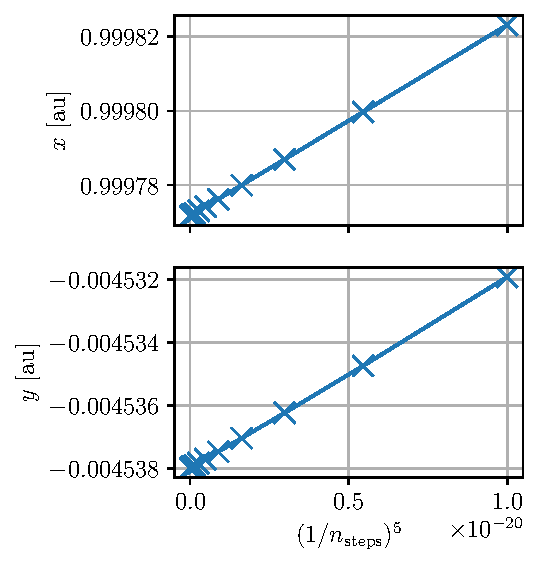
\includegraphics[width=\linewidth]{figures/lagrange_convergence_fixed.pdf}
        \caption{Fixed \(\dd t\) method}
        \label{fig:lagrange_conv_fixed}
    \end{subfigure}
    \begin{subfigure}{0.49\linewidth}
        \centering
        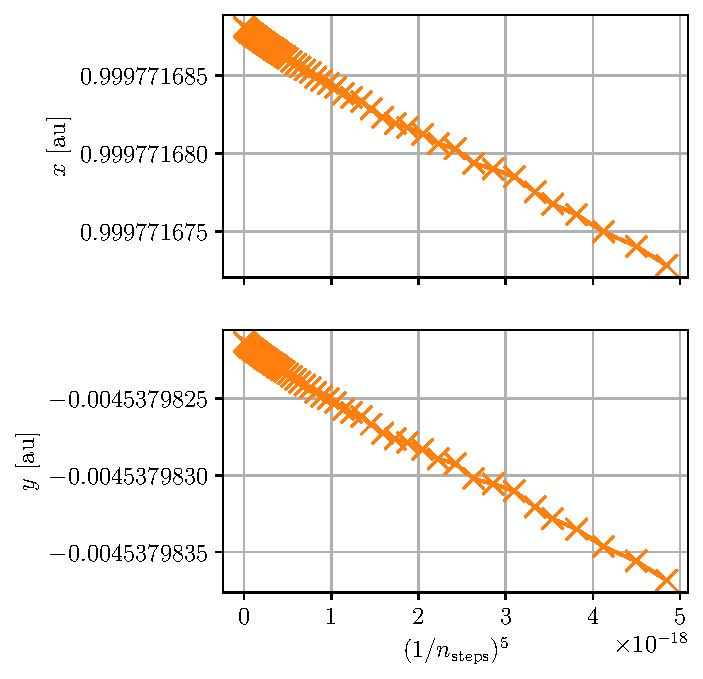
\includegraphics[width=\linewidth]{figures/lagrange_convergence_adapt.pdf}
        \caption{Adaptative \(\dd t\) method}
        \label{fig:lagrange_conv_adapt}
    \end{subfigure}
    \caption{Final position convergence starting from L2 with initial downwards speed \(\dot y' = -0.1\) m/s for both methods. \(n_\textrm{steps}\) was varied from \(10^4\) to \(10^6\) for the fixed timestep method and the tolerance \(\varepsilon\) was varied from \(10^{-5}\) to \(10^{-1}\) for the adaptative method.}
    \label{fig:lagrange_conv}
\end{figure}

Mechanical energy over time is shown in \autoref{fig:lagrange_emec}. Both methods seem to give similar energy levels. Error on conservation of mechanical energy for both methods is also given in \autoref{fig:lagrange_emec_error}. While both methods give a similar error, the initial spread is much smaller for adaptative method than the fixed one. While mechanical energy does not seem to be conserved well for each step, mechanical energy seems to recover after each bump, making it a bit more conserved overall. Analysing the location of the spikes in energy reveals that they occur at the intersection between the trajectory and the Earth-Sun axis (\(x'\) axis). This is shown in \autoref{fig:lagrange_max_mins_energy}. These locations corresponds to brutal changes in speed along the \(y'\) axis.

\begin{figure}[h]
    \centering
    \begin{minipage}{.45\textwidth}
        \centering
        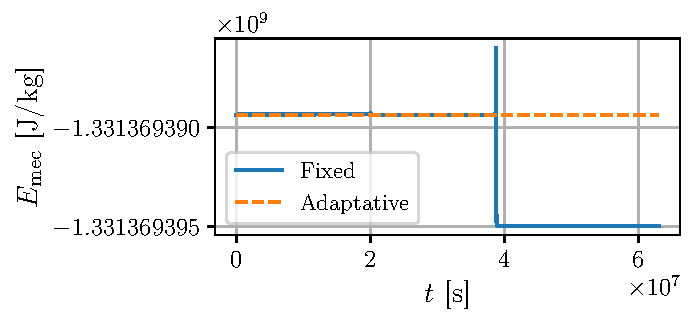
\includegraphics[width=\linewidth]{figures/lagrange_emec.pdf}
        \captionof{figure}{Mechanical energy over time for both methods}
        \label{fig:lagrange_emec}
    \end{minipage}
    \hspace*{1cm}
    \begin{minipage}{.45\textwidth}
        \centering
        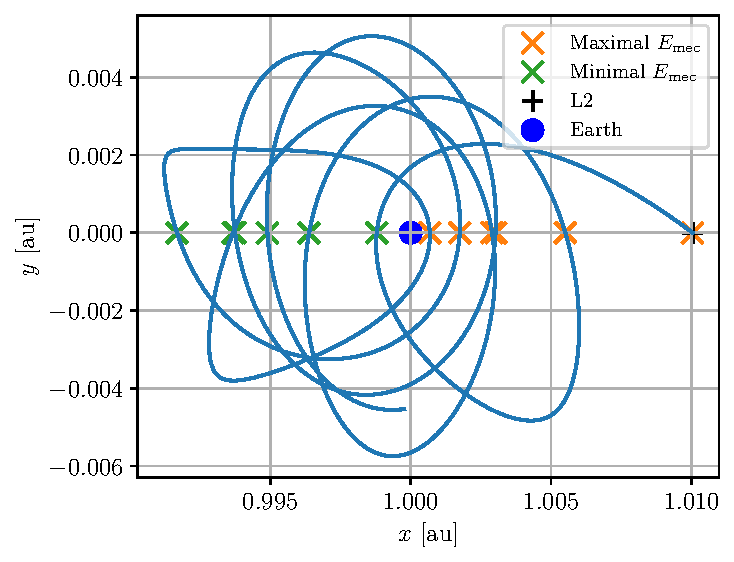
\includegraphics[width=\linewidth]{figures/lagrange_max_mins_energy.pdf}
        \captionof{figure}{Points on trajectory where mechanical energy is maximal or minimal, using adaptative method}
        \label{fig:lagrange_max_mins_energy}
    \end{minipage}
\end{figure}

\begin{figure}[h]
    \centering
    \begin{subfigure}{0.48\linewidth}
        \centering
        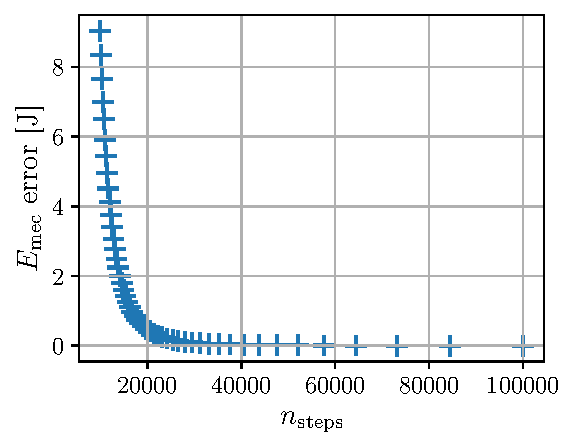
\includegraphics[width=\linewidth]{figures/lagrange_emec_error_fixed.pdf}
        \caption{Fixed \(\dd t\) method}
        \label{fig:lagrange_emec_error_fixed}
    \end{subfigure}
    \begin{subfigure}{0.48\linewidth}
        \centering
        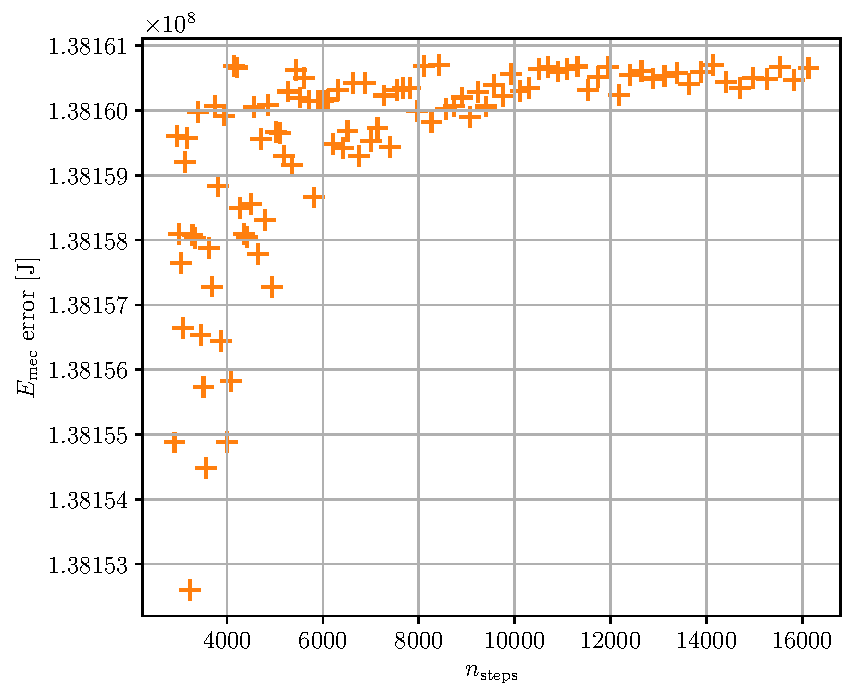
\includegraphics[width=\linewidth]{figures/lagrange_emec_error_adapt.pdf}
        \caption{Adaptative \(\dd t\) method}
        \label{fig:lagrange_emec_error_adapt}
    \end{subfigure}
    \caption{Mechanical energy error starting from L2 with initial downwards speed \(\dot y' = -0.1\) m/s for both methods. \(n_\textrm{steps}\) was varied from \(10^4\) to \(10^6\) for the fixed timestep method and the tolerance \(\varepsilon\) was varied from \(10^{-5}\) to \(10^{-1}\) for the adaptative method.}
    \label{fig:lagrange_emec_error}
\end{figure}

Let's analyse the trajectory more closely, specially the behavior near L2. Using the initial configuration given at the beginning of this section, we get the trajectory given in \autoref{fig:lagrange_trajectory}. Because of the initial perturbation, the satelite falls towards Earth and starts orbiting. It gets trapped in the potential field of the Earth, as is clearly shown in \autoref{fig:lagrange_trajectory_potential}. This result is expected because the Lagrange point L2 is unstable, as will be discussed later. The small downwards speed reduces the centrifugal force, which pushed the satelite away from Earth. A lower centrifugal force thus means that the satelite gets pulled towards Earth. If the initial speed was upwards, the satelite would get pushed away! The trajectory in \autoref{fig:lagrange_v0_up} shows this.

\begin{figure}[h]
    \centering
    \begin{subfigure}{0.46\linewidth}
        \centering
        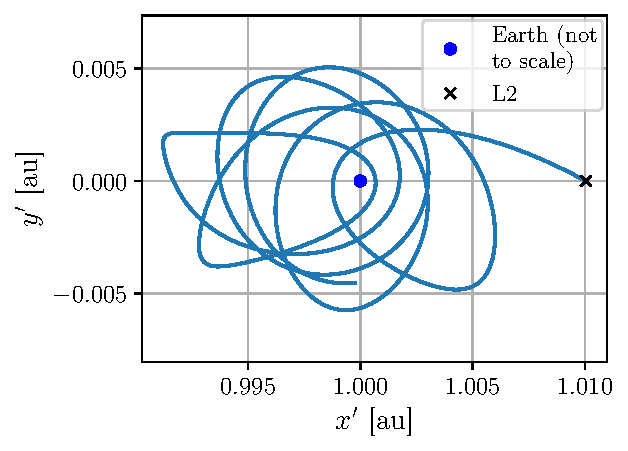
\includegraphics[width=\linewidth]{figures/lagrange_trajectory.pdf}
        \caption{Trajectory using adaptative method}
        \label{fig:lagrange_trajectory}
    \end{subfigure}
    \begin{subfigure}{0.53\linewidth}
        \centering
        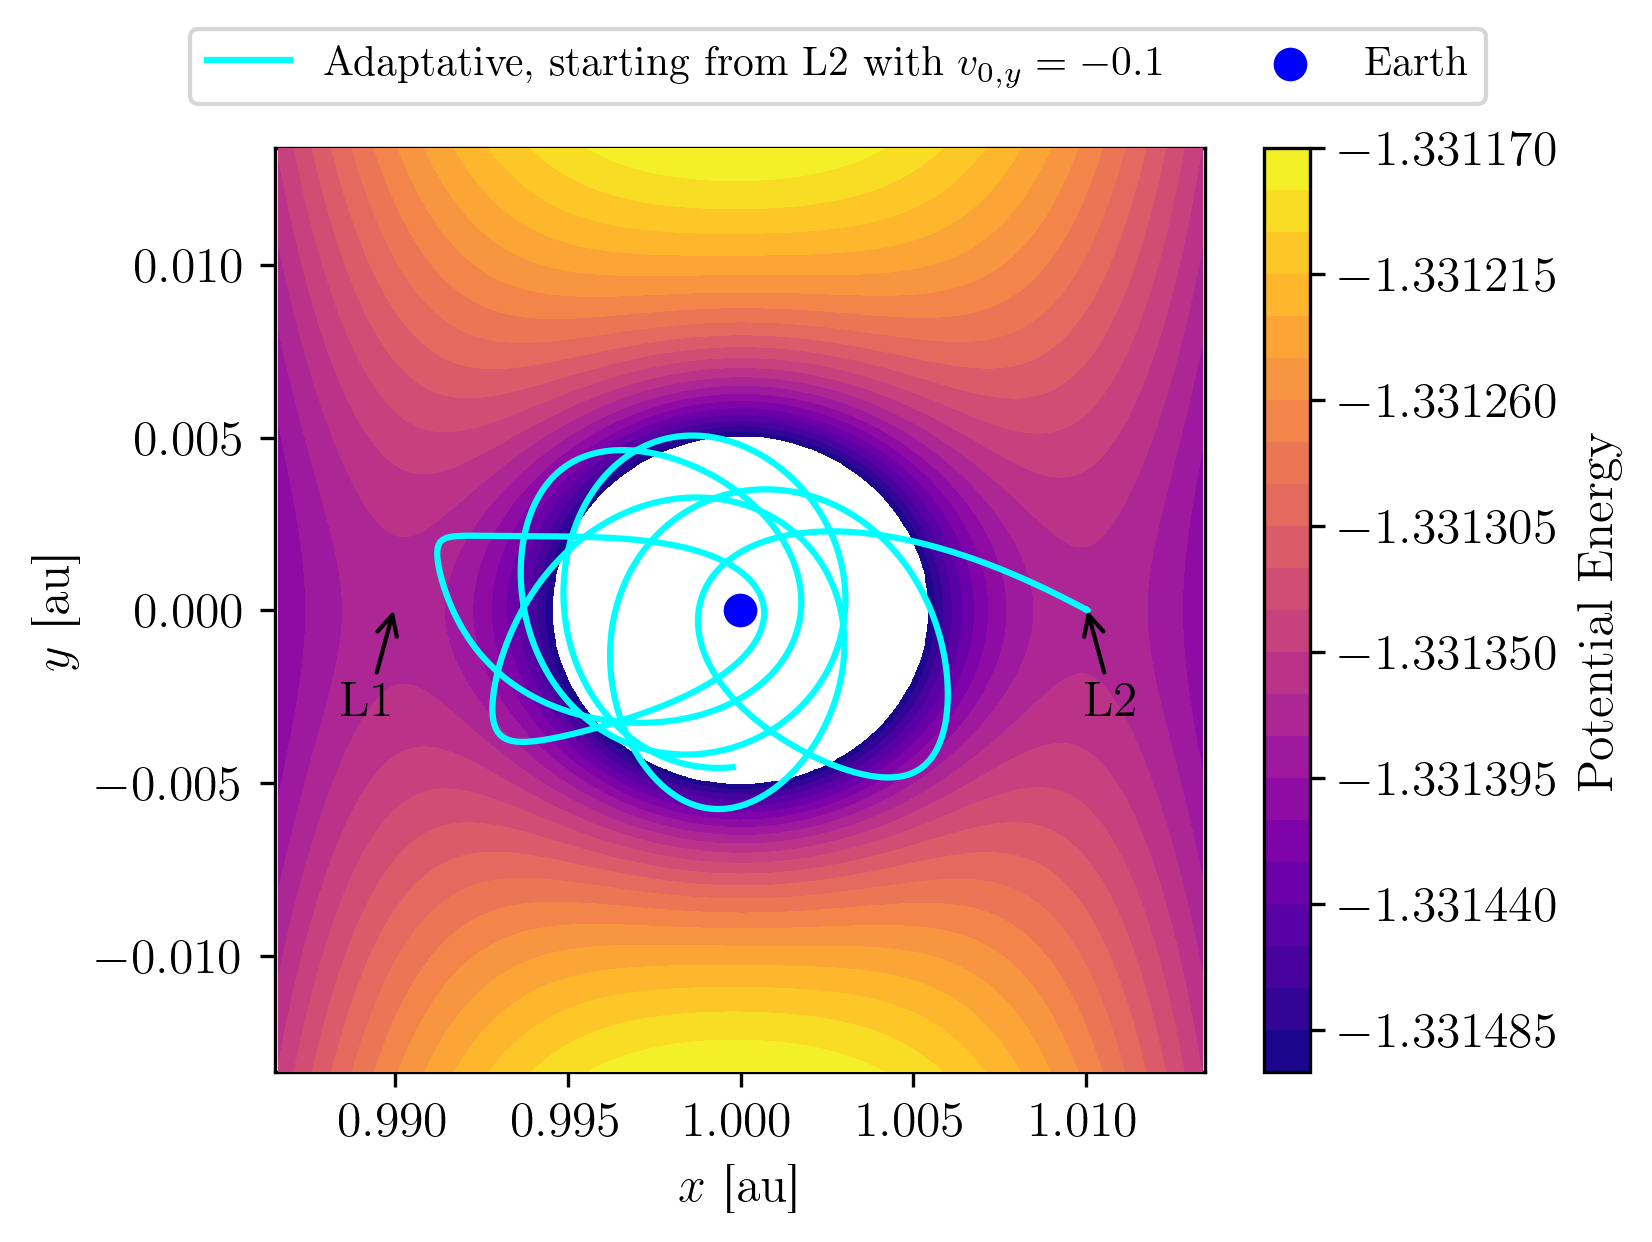
\includegraphics[width=\linewidth]{figures/potential_L1_L2_zoom_trajectory.png}
        \caption{Trajectory with potential}
        \label{fig:lagrange_trajectory_potential}
    \end{subfigure}
    \caption{Trajectory of Webb after falling in the potential well of the Earth}
\end{figure}

\begin{figure}[h]
    \centering
    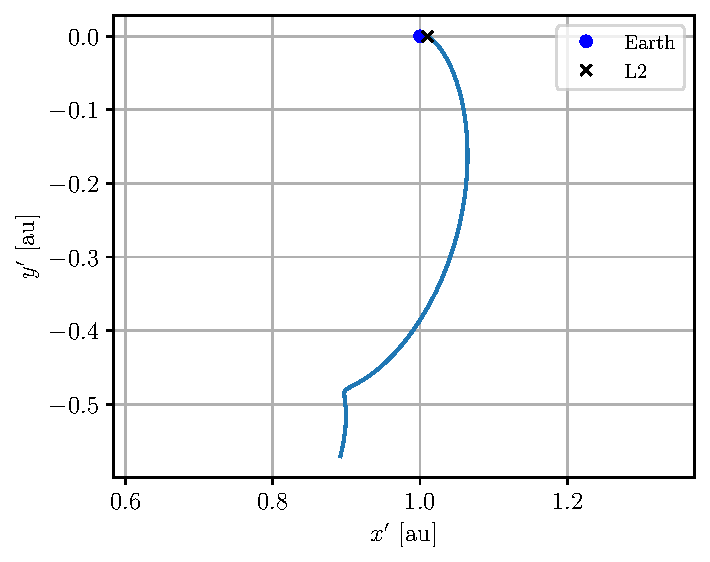
\includegraphics[width=0.6\linewidth]{figures/lagrange_v0_up.pdf}
    \caption{Trajectory starting from L2 with initial upwards speed \(\dot y' = 0.1\) m/s, using adaptative method with tolerance \(\varepsilon = 10^{-4}\)}
    \label{fig:lagrange_v0_up}
\end{figure}

It is interesting to note that the distance to L2 grows exponentially over time, for a given range. Indeed, \autoref{fig:lagrange_distance_L2} shows that this range is for \(t < 2 \cdot 10^7 \textrm{ s} \approx 231 \textrm{ days}\), after which the satelite remains far from L2.

\begin{figure}[h]
    \centering
    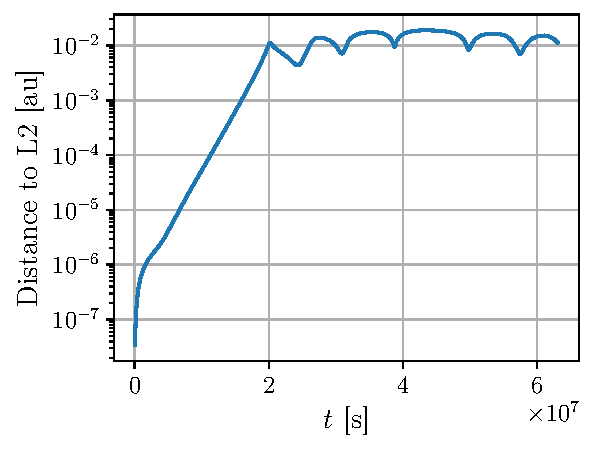
\includegraphics[width=0.6\linewidth]{figures/lagrange_exponential_distance.pdf}
    \caption{Distance from L2 over time, starting from L2 with initial downwards speed \(\dot y' = -0.1\)}
    \label{fig:lagrange_distance_L2}
\end{figure}

Let's study the potential energy a bit more closely, allowing us to find the stability of the Lagrange point L2 for example. At the scale of the solar system, we can identify a bump in the potential, which could hint at the presence of other Lagrange points. There is a ring where potential increases slightly, as shown in \autoref{fig:lagrange_potential_global}. While the scale of the figure does not show it, there should be saddle points and some wells allowing for other Lagrange points, whose locations are marked approximately on the figure \cite{lagrange}. Around the Earth, it is possible to see that the Lagrange points L1 and L2 are placed on saddle points, meaning they are unstable. \autoref{fig:lagrange_L1_L2}. This is coherent with what was observed in the simulations. Another visualisation of the potential is shown in \autoref{fig:lagrange_potential_3D}.

\begin{figure}[h]
    \centering
    \begin{subfigure}{0.48\linewidth}
        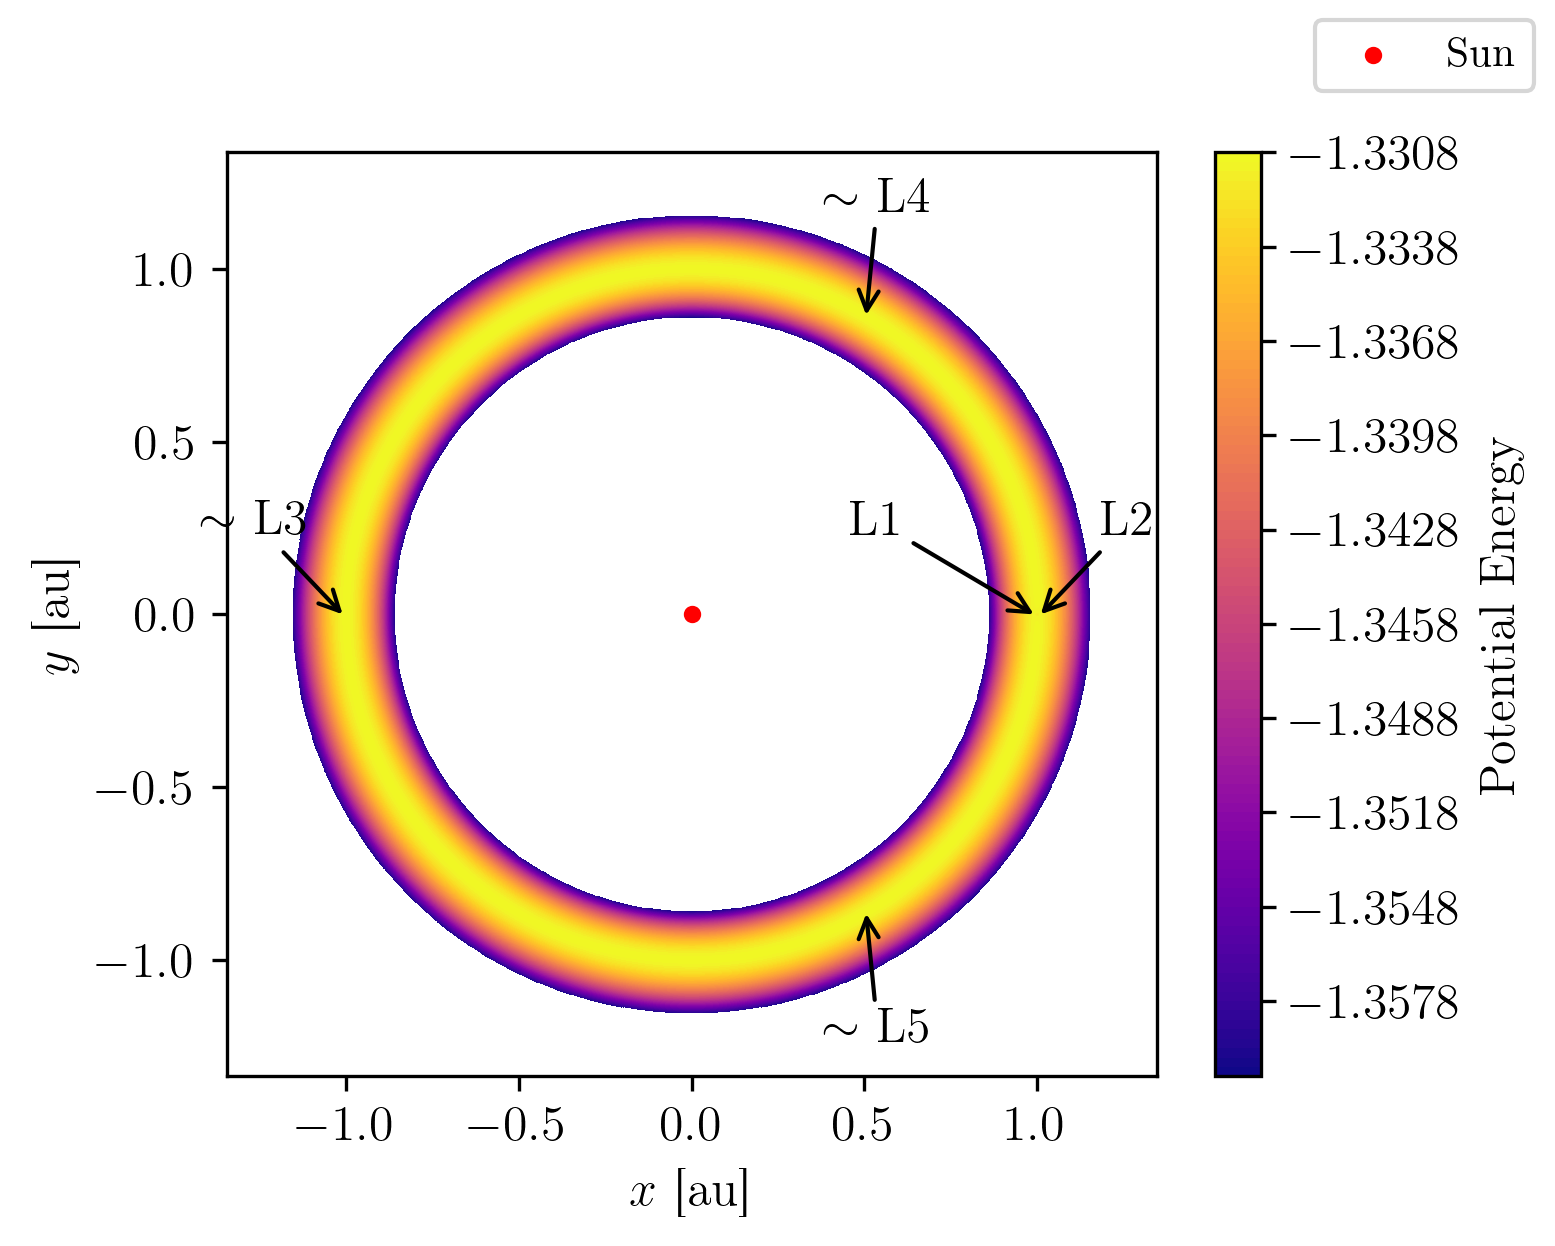
\includegraphics[width=\linewidth]{figures/potential_global.png}
        \caption{Potential energy band for a distance around the Sun-Earth distance.}
        \label{fig:lagrange_potential_global}
    \end{subfigure}
    \begin{subfigure}{0.48\linewidth}
        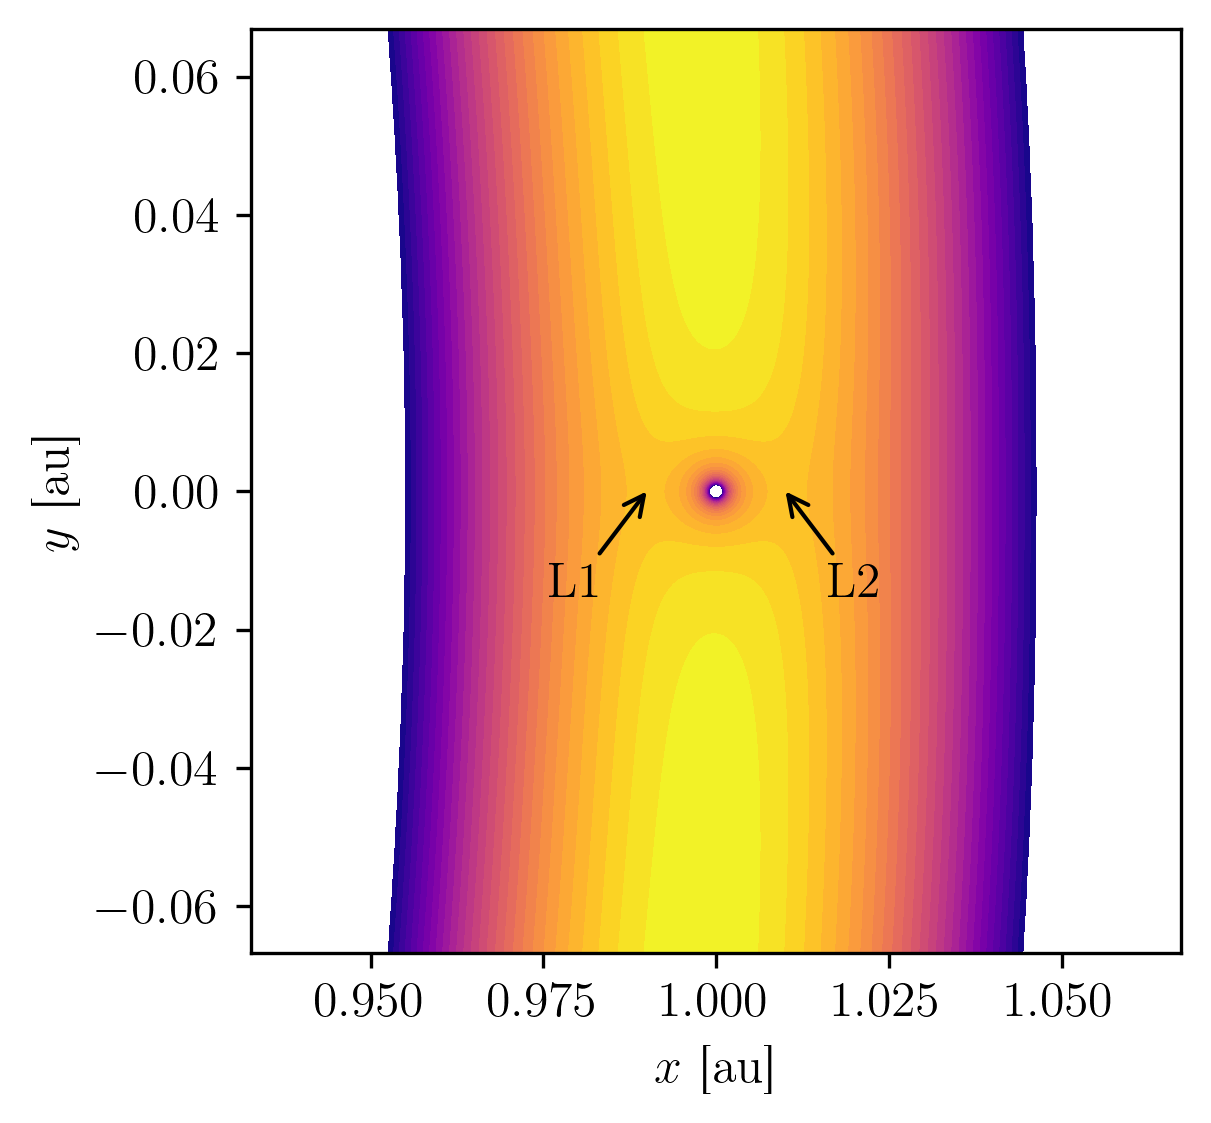
\includegraphics[width=\linewidth]{figures/potential_L1_L2_zoom.png}
        \vspace*{0.2cm}
        \caption{Potential energy around Earth}
        \label{fig:lagrange_L1_L2}
    \end{subfigure}
    \caption{Potential energy at different points in the Sun-Earth system}
\end{figure}

\begin{figure}[h]
    \centering
    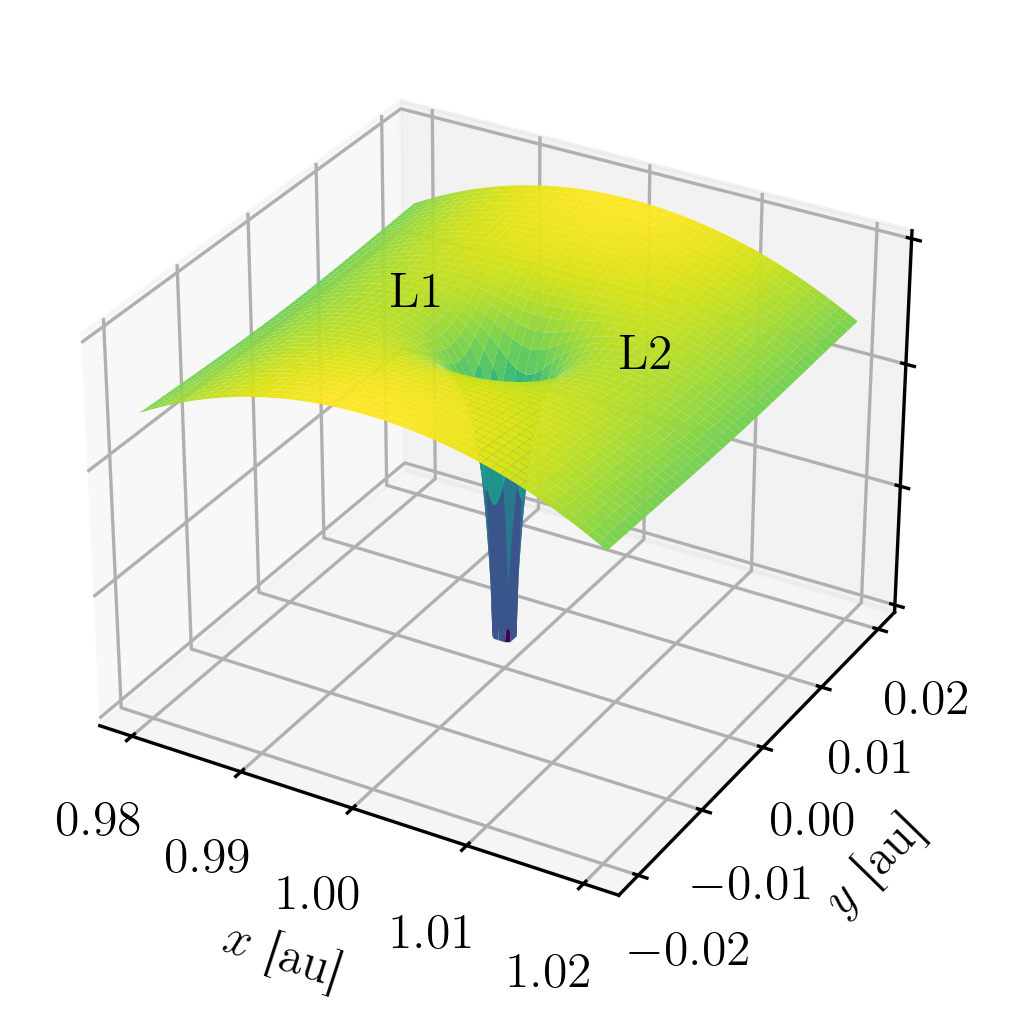
\includegraphics[width=0.6\linewidth]{figures/potential3D_L1_L2_zoom.png}
    \caption{3D representation of the potential around Earth}
    \label{fig:lagrange_potential_3D}
\end{figure}